\documentclass[titlepage,a4paper]{article}

\usepackage{a4wide}
\usepackage[colorlinks=true,linkcolor=black,citecolor=black,urlcolor=blue,bookmarksopen=true]{hyperref}
\usepackage{bookmark}
\usepackage{fancyhdr}
\usepackage[spanish,es-tabla,es-nodecimaldot]{babel}
\usepackage[utf8]{inputenc}
\usepackage[T1]{fontenc}
\usepackage{lmodern}
\usepackage{microtype}
\usepackage{graphicx}
\usepackage{float}
\usepackage{caption}
\captionsetup{font=small,labelfont=bf}
\captionsetup[table]{name=Tabla}
\usepackage{booktabs}
\usepackage{tabularx}
\usepackage{array}
\usepackage{amsmath}
\usepackage[table]{xcolor}
\graphicspath{{figuras/}}
\emergencystretch=3em

\newcolumntype{Y}{>{\centering\arraybackslash}X}
\newcommand{\code}[1]{\texttt{#1}}

\pagestyle{fancy} % Encabezado y pie de página
\fancyhf{}
\fancyhead[L]{TP1 - Deserción universitaria}
\fancyhead[R]{Aprendizaje Automático}
\renewcommand{\headrulewidth}{0.4pt}
\fancyfoot[C]{\thepage}
\renewcommand{\footrulewidth}{0.4pt}
\setlength{\headheight}{14pt}

\begin{document}
\begin{titlepage} % Carátula
    \vspace*{\fill}
    \centering
    
\includegraphics[width=\textwidth]{Logo_UBA_2.png}

    \vspace*{\fill}
    \vfill
    {\Huge \textbf{Predicción de la deserción en estudiantes universitarios con modelos clásicos de aprendizaje automático}\par}
    \vskip2cm
    \Large Aprendizaje Automático\\
    Trabajo práctico 1 \\
    Comisión 2 \\
    Segundo cuatrimestre de 2026
    \vfill
    \vfill

    Alumnos: \\
    Martín López\\
    Diego Alejandro Rojas Betancourt

    \vspace*{\fill}
\end{titlepage}

\newpage
% =====================================================================
\section*{Resumen}

La deserción universitaria tiene altos costos personales e institucionales. Este trabajo, con 49.687 registros de una institución de educación superior, persigue tres objetivos: (i) predecir la deserción al cierre del primer año para aplicar el modelo a los estudiantes que siguen cursando, (ii) distinguir los tres estados académicos (desertor, en curso, graduado) y (iii) explicar qué factores se asocian al abandono. En la tarea binaria, entrenada solo con estudiantes de desenlace conocido (graduados y desertores), regresión logística, SVM, árbol de decisión y un ensamble \textit{Voting} alcanzaron un F1-macro de 0,936--0,939 y un AUC de 0,968--0,976 en prueba; aplicado a los estudiantes en curso, el modelo asigna probabilidad alta de deserción ($\geq 0{,}8$) al 26\,\%. En la tarea multiclase, XGBoost obtuvo el mejor F1-macro (0,789), pero la clase ``en curso'' fue la más difícil de reconocer. Las curvas de complejidad mostraron sobreajuste en árboles profundos, SVM con $\gamma$ alto y K-NN con $k$ pequeño. Una regresión logística explicativa con 10 de 20 predictores y un índice de rendimiento académico mantuvo un AUC de 0,970 e identificó al rendimiento académico y a la morosidad en la matrícula como los factores más asociados a la deserción.

% =====================================================================
\section{Introducción}\label{sec:introduccion}

El abandono de los estudios universitarios es uno de los problemas más persistentes de la educación superior: implica una pérdida de recursos para las instituciones y consecuencias de largo plazo para los estudiantes. Este trabajo aborda la deserción al finalizar el primer año con tres objetivos complementarios: \textbf{predecir} el riesgo de abandono para que las áreas responsables puedan planificar acciones de acompañamiento; \textbf{distinguir} los tres estados académicos (graduado, desertor y en curso); y \textbf{comprender} qué factores se asocian con la deserción. Esperamos que las variables de rendimiento académico del primer año sean las más relevantes, seguidas por la situación financiera (pago de la matrícula, deuda, beca). El problema se aborda con modelos clásicos de clasificación supervisada.

La literatura teórica (Tinto, 1975, 1993; Bean, 1980; Bean y Metzner, 1985) y empírica (Yorke y Longden, 2004; OECD, 2019) caracteriza la deserción como un fenómeno multicausal, ligado a la integración académica y social del estudiante y a factores externos como los financieros. El conjunto de datos de referencia fue publicado por Realinho et al.\ (2022) con el fin explícito de construir modelos de alerta temprana, y trabajos previos (Martins et al., 2021; Kim et al., 2023) señalan a las unidades aprobadas como predictor dominante, pero suelen usar un único esquema de clasificación o no indican cómo tratar a los estudiantes que siguen cursando, cuyo desenlace todavía se desconoce. El \textit{gap} que buscamos cubrir es separar con claridad la tarea predictiva (entrenada con desenlaces conocidos y aplicada a los estudiantes en curso) de la descriptiva (multiclase) y de la explicativa, y analizar la \textbf{capacidad de generalización} de los modelos mediante curvas de complejidad.

La pregunta que guía el estudio es: \textbf{¿cómo permiten las variables disponibles al finalizar el primer año estimar el riesgo de deserción, distinguir la categoría ``en curso'' y comprender los factores asociados al abandono?} Planteamos que (H1) el rendimiento académico concentra la mayor parte del poder predictivo, seguido por la situación financiera; (H2) en la tarea binaria un modelo lineal regularizado alcanza el desempeño de modelos no lineales, por lo que puede usarse a la vez para predecir y para explicar; y (H3) en la tarea multiclase los ensambles de árboles superan a los modelos individuales, siendo ``en curso'' la clase más difícil. En la Sección~\ref{sec:metodos} se describen los datos y métodos; en la Sección~\ref{sec:resultados}, los resultados; en la Sección~\ref{sec:discusion}, sus implicancias y limitaciones; y en la Sección~\ref{sec:conclusion}, las conclusiones.

% =====================================================================
\section{Materiales y métodos}\label{sec:metodos}

\subsection{Datos y variables explicativas (E)}

Se utilizó el archivo provisto por la cátedra (\code{dataset\_TP1\_2026.csv}), una versión ajustada del dataset aumentado sintéticamente de Kaggle (Playground Series S4E6; Reade y Chow, 2024), generado a partir del dataset de UCI de Realinho et al.\ (2022). Contiene 50.000 registros y 27 atributos más la variable objetivo, sin valores faltantes. Se eliminaron \textbf{313 filas duplicadas} (idénticas en todas las columnas, producto de la aumentación) para que un mismo registro no quede a la vez en entrenamiento y prueba; la muestra final tiene \textbf{49.687 estudiantes}. Los atributos se agrupan en: (i) \textbf{inscripción y demografía} (edad, sexo, estado civil, carrera, turno, modo de acceso, estudios previos y su nota, puntaje de ingreso, desplazado, internacional, necesidades educativas especiales); (ii) \textbf{socioeconómicos} (deuda, matrícula al día, beca y nivel de la ocupación de cada progenitor); y (iii) \textbf{académicos del primer año} (unidades curriculares ---UC--- inscriptas, evaluadas y aprobadas y nota promedio de cada semestre). Se asume que todas estas variables están disponibles al cierre del primer año y que la variable objetivo es el desenlace posterior.

Al revisar la construcción de las variables se encontró que \code{Ingresos\_Padre/Madre} y \code{Demanda\_Cog\_Padre/Madre} se derivan con la misma regla ISCO-08 y tienen una \textbf{correspondencia 1 a 1}: son la misma variable con otra etiqueta, por lo que se conservó una sola. Las variables académicas de ambos semestres están muy correlacionadas ($\rho \approx 0{,}8$--$0{,}9$). Para las tareas binaria y explicativa se construyeron \textbf{variables derivadas}: indicadores 0/1, promedios de los dos semestres (notas, UC inscriptas, UC aprobadas y evaluaciones), la \textbf{tasa de aprobación} (UC aprobadas / UC inscriptas), el nivel ocupacional promedio de la familia y macro-categorías de carrera (6 áreas), estado civil y estudios previos. Como posibles sesgos, se trata de una única institución, con datos aumentados sintéticamente y con atributos muy desbalanceados (p.\ ej., 99\,\% de estudiantes no internacionales).

\textbf{Preprocesamiento.} Las variables categóricas se codificaron \textit{one-hot} y las numéricas se estandarizaron (necesario para la regularización de la regresión logística y para los modelos basados en distancias, como SVM y K-NN). Todo el preprocesamiento se incluyó en un \code{Pipeline} de scikit-learn, que se ajusta solo con los datos de entrenamiento de cada \textit{fold}, sin fuga de información.

\subsection{Variable respuesta y tarea objetivo (T)}

La variable \code{target} tiene tres estados: Graduado (47,3\,\%), Desertor (33,0\,\%) y En curso (19,6\,\%) (Figura~\ref{fig:clases}). En la \textbf{tarea binaria} se usaron únicamente los estudiantes con desenlace conocido, \textbf{Graduado (0) vs.\ Desertor (1)} (39.925 registros; 41,1\,\% desertores), y se \textbf{excluyeron los ``en curso''}: como todavía no se sabe si se graduarán o abandonarán, incluirlos como ``no desertores'' contaminaría la etiqueta. El modelo entrenado se aplica luego a esos 9762 estudiantes para estimar su riesgo de deserción. En la \textbf{tarea multiclase} se usaron los tres estados. El desbalance es moderado, por lo que no se aplicó sobre-muestreo: se usaron particiones estratificadas y el \textbf{F1-macro} (promedio no ponderado del F1 de cada clase) para seleccionar y comparar modelos; en la multiclase se exploró además \code{class\_weight = "balanced"} como hiper-parámetro.

\subsection{Manejo de datos y esquemas de clasificación}

\textbf{Clasificación binaria.} Partición estratificada 80/20 (31.940 registros de entrenamiento y 7985 de prueba). Se entrenaron regresión logística (LR), SVM con kernel RBF y árbol de decisión sobre las variables derivadas; los hiper-parámetros se eligieron por búsqueda en grilla con validación cruzada (CV) estratificada de 5 \textit{folds} maximizando el F1-macro (Tabla~\ref{tab:hiperparametros}). Como el costo de la SVM con kernel crece con el cuadrado del número de muestras, su grilla se evaluó en una submuestra estratificada de 10.000 registros y el modelo final se reentrenó con todo el entrenamiento. Con los tres modelos se construyó un ensamble \textbf{Voting} \textit{hard} (mayoría de votos) y \textit{soft} (promedio de probabilidades; para la SVM, escalado de Platt). Como referencia se agregó Gradient Boosting con los hiper-parámetros de una búsqueda preliminar.

\textbf{Clasificación multiclase.} Nueva partición estratificada 80/20 con otra semilla (39.749 / 9938), sobre las 25 variables originales (47 atributos codificados). Se entrenaron K-NN y árbol de decisión, y los ensambles Random Forest (\textit{bagging}; Breiman, 2001), AdaBoost y XGBoost (\textit{boosting}); como referencia lineal, una regresión logística multinomial y su variante \textit{one-vs-rest} (OvR). K-NN y los árboles son \textbf{intrínsecamente multiclase} (estiman la proporción de cada clase en el vecindario u hoja), AdaBoost usa la variante SAMME y XGBoost una pérdida \textit{softmax}. La selección se hizo con CV de 5 \textit{folds} maximizando el F1-macro.

\begin{table}[!htbp]
\centering
\caption{Hiper-parámetros explorados y valores seleccionados por validación cruzada}
\label{tab:hiperparametros}
\footnotesize
\renewcommand{\arraystretch}{1.12}
\begin{tabularx}{\textwidth}{@{}>{\raggedright\arraybackslash}p{2.6cm} >{\raggedright\arraybackslash}X >{\raggedright\arraybackslash}p{3.3cm} >{\centering\arraybackslash}p{2.3cm}@{}}
\toprule
\textbf{Esquema / modelo} & \textbf{Hiper-parámetros y rangos explorados} & \textbf{Valores seleccionados} & \textbf{F1-macro CV (media $\pm$ sd)} \\
\midrule
Bin. -- Reg.\ logística & $C \in \{0{,}001; 0{,}01; 0{,}1; 1; 10; 100\}$; penalización L1, L2 o \textit{elastic net} (\code{l1\_ratio} $\in \{0{,}1; 0{,}5; 0{,}9\}$) & \textit{elastic net}; $C = 0{,}1$; \code{l1\_ratio} $= 0{,}5$ & $0{,}939 \pm 0{,}003$ \\
Bin. -- SVM (RBF) & $C \in \{0{,}1; 1; 10; 100\}$; $\gamma \in \{0{,}003; 0{,}01; 0{,}03; 0{,}1\}$ & $C = 100$; $\gamma = 0{,}003$ & $0{,}939 \pm 0{,}004$\textsuperscript{*} \\
Bin. -- Árbol & \code{max\_depth} $\in \{3; 5; 10; 20; \text{None}\}$; \code{min\_samples\_split} $\in \{2; 5; 10\}$; \code{min\_samples\_leaf} $\in \{1; 2; 4\}$; gini/entropía & prof.\ = 5; hoja $\geq$ 4; gini & $0{,}937 \pm 0{,}002$ \\
\midrule
Multi -- K-NN & $k \in \{5; 11; 21; 41; 61; 101\}$; pesos uniforme/distancia; métrica euclídea/Manhattan & $k = 21$; uniforme; Manhattan & $0{,}759 \pm 0{,}005$ \\
Multi -- Árbol & \code{max\_depth} $\in \{4;\dots;20\}$; \code{min\_samples\_leaf} $\in \{1; 10; 50; 100\}$; gini/entropía; \code{class\_weight} & prof.\ = 8; hoja $\geq$ 1; gini; sin pesos & $0{,}775 \pm 0{,}005$ \\
Multi -- Reg.\ log.\ multinomial & $C \in \{0{,}01; 0{,}1; 1; 10\}$; \code{class\_weight} & $C = 1$; balanced & $0{,}781 \pm 0{,}005$ \\
Multi -- Random Forest & 200 árboles; \code{max\_depth} $\in$ \{12; 20; None\}; \code{max\_features} $\in \{\sqrt{p}; 0{,}3\}$; \code{min\_samples\_leaf} $\in \{1; 5\}$; \code{class\_weight} & prof.\ = 20; $\sqrt{p}$; hoja $\geq$ 1; balanced & $0{,}789 \pm 0{,}005$ \\
Multi -- AdaBoost & 200 estimadores; \code{learning\_rate} $\in \{0{,}1; 0{,}5; 1\}$; prof.\ árbol base $\in \{1; 2; 3\}$ & $\eta = 1{,}0$; prof.\ base = 3 & $0{,}783 \pm 0{,}004$ \\
Multi -- XGBoost & \code{n\_estimators} $\in \{200; 500\}$; \code{learning\_rate} $\in \{0{,}05; 0{,}1\}$; \code{max\_depth} $\in \{3; 5; 7\}$; \code{subsample} = \code{colsample\_bytree} = 0{,}8 & 500 árboles; $\eta = 0{,}05$; prof.\ = 5 & $0{,}790 \pm 0{,}004$ \\
\bottomrule
\end{tabularx}

\vspace{2pt}
\begin{minipage}{\textwidth}\scriptsize
Búsqueda en grilla con CV estratificada de 5 \textit{folds} sobre el entrenamiento. Bin.\ = binaria (Graduado vs.\ Desertor); Multi = multiclase; sd = desvío estándar entre \textit{folds}; prof.\ = profundidad máxima; $\eta$ = tasa de aprendizaje; $p$ = número de atributos. \textsuperscript{*}Submuestra de 10.000 registros. Gradient Boosting (referencia binaria): 200 árboles, $\eta = 0{,}1$, prof.\ = 3, \code{subsample} = 0{,}8.
\end{minipage}
\end{table}

\subsection{Evaluación de modelos}

Cada modelo final se evaluó una única vez en el conjunto de prueba con accuracy, precisión, recall, F1, F1-macro y AUC-ROC (en la multiclase, versiones \textit{macro} y AUC \textit{one-vs-rest}). Las \textbf{curvas de complejidad} se construyeron con \code{validation\_curve} (CV de 5 \textit{folds}, nunca con el test), variando el hiper-parámetro que controla la complejidad con los demás en su valor óptimo. La importancia de atributos se estimó por \textbf{permutación} en el conjunto de prueba; como esta medida subestima las variables correlacionadas ---al permutar una, el modelo usa la información de otra---, también se permutaron \textbf{grupos de variables} formados por clustering jerárquico sobre la correlación de Spearman ($|\rho| > 0{,}5$). Se trabajó en Python con pandas, scikit-learn (Pedregosa et al., 2011), xgboost (Chen y Guestrin, 2016) y statsmodels; todas las semillas se fijaron en 42.

\subsection{Modelo explicativo}\label{sec:met_explicativo}

Para interpretar la asociación de cada factor con la deserción se ajustó una regresión logística sobre la partición binaria, con un \textbf{conjunto reducido de predictores} que evita la multicolinealidad: macro-categorías, sin variables redundantes (p.\ ej., se excluyó la deuda, correlacionada con la morosidad) y con un \textbf{índice de rendimiento académico} que promedia el promedio de notas y la tasa de aprobación, estandarizados con la media y el desvío del entrenamiento. Las variables continuas se estandarizaron y los indicadores 0/1 se dejaron en su escala. La regularización L1 (Lasso) se eligió por CV con la \textbf{regla de 1 error estándar} (el $C$ más chico cuyo F1-macro de validación queda a menos de un error estándar del máximo). Con las variables retenidas se reajustó una regresión logística sin penalización (statsmodels) para obtener \textit{odds ratios} (OR), intervalos de confianza al 95\,\% (IC) y valores p, y se verificó el factor de inflación de la varianza (VIF). Como análisis previo se calculó el \textbf{Valor de Información} (IV) de cada variable sobre el entrenamiento binario: $\mathrm{IV} = \sum_i (\%\,\text{graduados}_i - \%\,\text{desertores}_i)\,\ln(\%\,\text{graduados}_i / \%\,\text{desertores}_i)$, con deciles para las numéricas; por convención, un IV $> 0{,}5$ es sospechosamente alto. El efecto del rendimiento sobre la probabilidad predicha se describió con gráficos de \textbf{dependencia parcial} (PDP) abiertos por variables categóricas.

% =====================================================================
\section{Resultados}\label{sec:resultados}

\subsection{Análisis exploratorio}

\begin{figure}[!htbp]
\centering
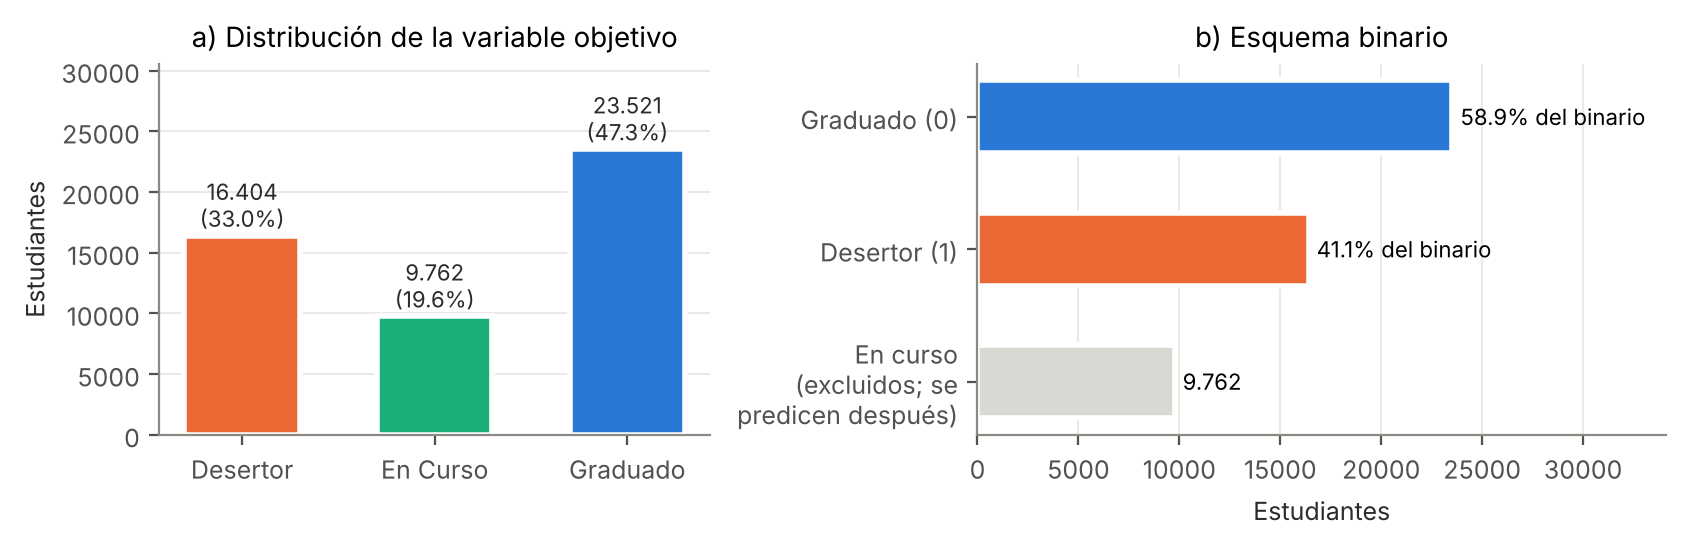
\includegraphics[width=0.72\textwidth]{fig1_clases.png}
\caption{\label{fig:clases}Distribución de la variable objetivo. (a) Esquema multiclase; número de estudiantes y porcentaje. (b) Esquema binario: se entrena con graduados y desertores; los estudiantes en curso se excluyen y se predicen después. $n = 49.687$ tras eliminar duplicados.}
\end{figure}

La Tabla~\ref{tab:iv} resume el poder de separación de cada variable entre graduados y desertores. Las variables académicas ---tasa de aprobación, UC aprobadas y promedio de notas--- tienen IV entre 4,3 y 5,2, muy por encima del umbral de 0,5; también lo superan las evaluaciones, la morosidad (1,44), la beca, la carrera, la edad, el modo de acceso y el sexo. Valores tan altos no implican fuga de información en sentido estricto ---las variables se registran durante el primer año---, pero indican que algunas son casi una manifestación de la deserción (Sección~\ref{sec:discusion}). El análisis descriptivo muestra el mismo patrón: el 68\,\% de los desertores no aprobó ninguna UC en el 2.\textsuperscript{o} semestre, y la tasa de deserción es de 93,9\,\% entre quienes no tienen la matrícula al día (25,7\,\% entre quienes sí), de 75,7\,\% entre quienes tienen deuda y de solo 7,2\,\% entre los becados. Graduados y estudiantes en curso se superponen bastante, lo que anticipa la dificultad de la tarea multiclase.

\begin{table}[!htbp]
\centering
\caption{Valor de Información (IV) de las 12 variables con mayor IV para distinguir graduados de desertores}
\label{tab:iv}
\small
\begin{tabular}{lc@{\hspace{1cm}}lc}
\toprule
\textbf{Variable} & \textbf{IV} & \textbf{Variable} & \textbf{IV} \\
\midrule
Tasa de aprobación (aprob./inscr.) & 5,20 & Carrera & 0,88 \\
UC aprobadas (prom.\ semestres) & 4,92 & Edad al inscribirse & 0,86 \\
Nota promedio (prom.\ semestres) & 4,27 & Modo de acceso & 0,63 \\
Evaluaciones (prom.\ semestres) & 1,50 & Sexo masculino & 0,58 \\
Moroso (matrícula no al día) & 1,44 & UC inscriptas (prom.\ semestres) & 0,55 \\
Becado & 0,96 & Tiene deuda & 0,35 \\
\bottomrule
\end{tabular}

\vspace{2pt}
{\scriptsize Calculado sobre el entrenamiento binario ($n = 31.940$); numéricas agrupadas en deciles. Convención: IV $< 0{,}02$ nulo; 0,02--0,1 débil; 0,1--0,3 medio; 0,3--0,5 fuerte; $> 0{,}5$ sospechosamente alto. UC = unidades curriculares.\par}
\end{table}



\subsection{Clasificación binaria: graduado vs.\ desertor}\label{sec:binaria}

La Tabla~\ref{tab:binaria} muestra que los tres modelos base alcanzan un desempeño casi idéntico en prueba (F1-macro de 0,936 a 0,938; AUC de 0,968 a 0,976), coherente con los valores de CV de la Tabla~\ref{tab:hiperparametros}. La \textbf{regresión logística} obtiene el mayor AUC y recall entre los modelos pedidos, y la \textbf{SVM}, la mayor precisión. El \textbf{Voting soft} logra el mejor F1-macro (0,939), igual al de Gradient Boosting, pero la mejora sobre la LR (0,002) es menor que el desvío entre \textit{folds}: las probabilidades de los tres modelos están muy correlacionadas ($r$ = 0,985--0,989) y solo discrepan en el 2,9\,\% de los casos de prueba, por lo que el ensamble tiene poca diversidad que aprovechar. El \textit{hard voting} tiene un AUC menor (0,946) porque solo produce cuatro niveles de puntaje (fracción de votos). La matriz de confusión del Voting soft (Figura~\ref{fig:roc}b) muestra que se identifica correctamente al 90,3\,\% de los desertores y al 96,9\,\% de los graduados.

\begin{table}[!htbp]
\centering
\caption{Desempeño de los modelos binarios (graduado vs.\ desertor) en el conjunto de prueba}
\label{tab:binaria}
\small
\begin{tabular}{lccccc}
\toprule
\textbf{Modelo} & \textbf{Accuracy} & \textbf{F1-macro} & \textbf{Precisión (des.)} & \textbf{Recall (des.)} & \textbf{AUC} \\
\midrule
Regresión logística      & 0,939 & 0,937 & 0,941 & \textbf{0,910} & \textbf{0,976} \\
SVM (RBF)                & 0,940 & 0,938 & \textbf{0,956} & 0,896 & 0,973 \\
Árbol de decisión        & 0,939 & 0,936 & 0,948 & 0,900 & 0,968 \\
Voting (soft)            & \textbf{0,942} & \textbf{0,939} & 0,953 & 0,903 & \textbf{0,976} \\
Voting (hard)            & 0,941 & 0,938 & 0,953 & 0,900 & 0,946 \\
\midrule
\textit{Gradient Boosting (ref.)} & \textit{0,942} & \textit{0,939} & \textit{0,944} & \textit{0,912} & \textit{0,978} \\
\bottomrule
\end{tabular}

\vspace{2pt}
{\scriptsize Clase positiva = Desertor (des.). $n_{\text{test}} = 7985$ (41\,\% desertores). Umbral 0,5. Voting (hard): AUC calculado con la fracción de votos. En negrita, el mejor valor entre los modelos pedidos por la consigna.\par}
\end{table}

\begin{figure}[!htbp]
\centering
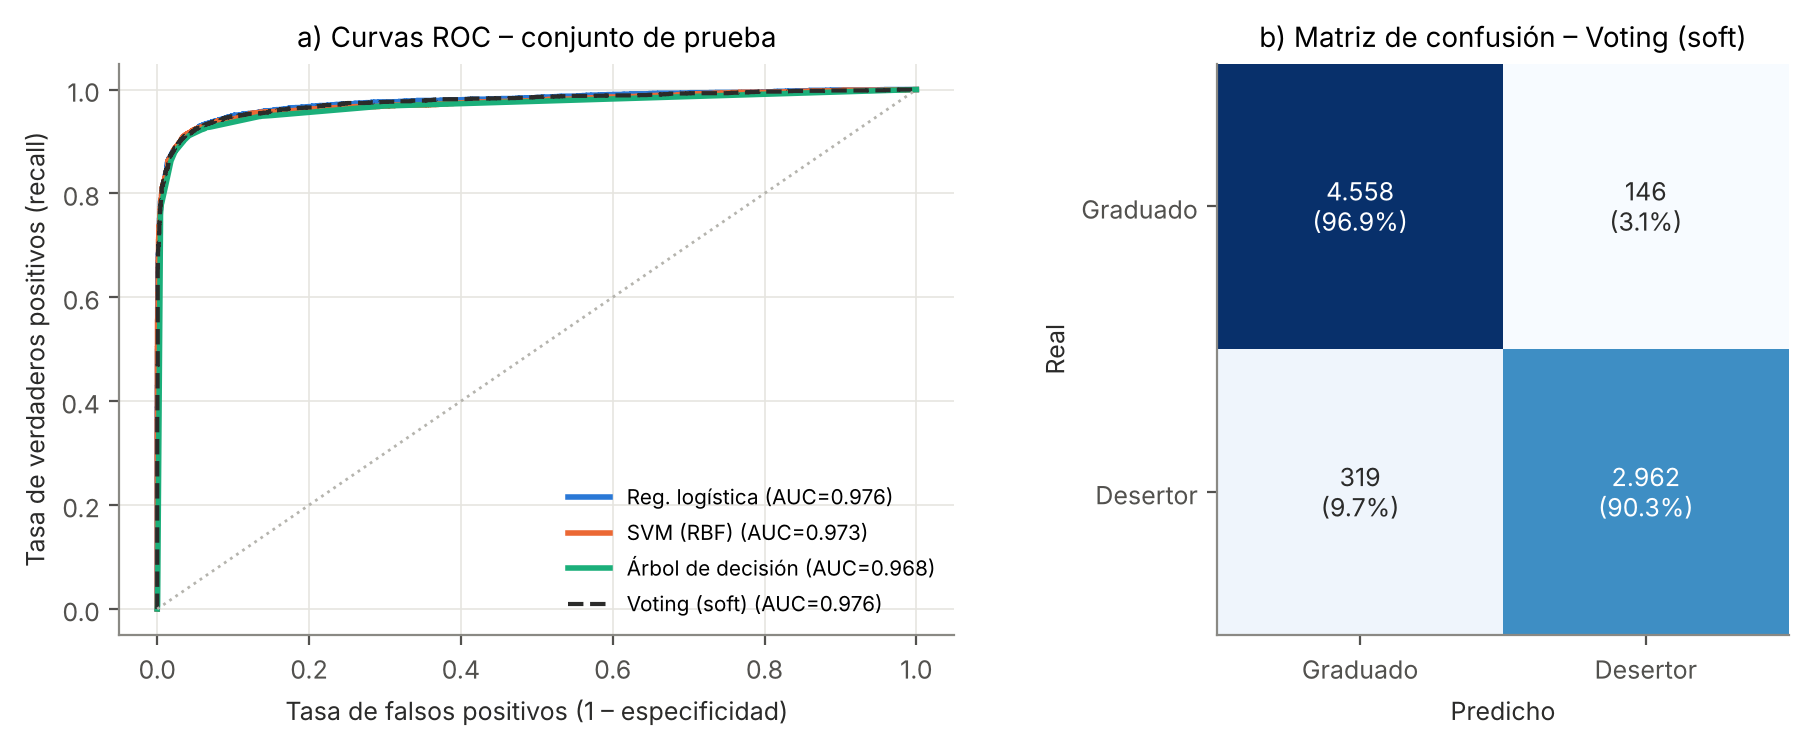
\includegraphics[width=0.78\textwidth]{fig3_roc_cm_bin.png}
\caption{\label{fig:roc}Curvas ROC y matriz de confusión del esquema binario. (a) Curvas ROC en prueba; la línea punteada corresponde a un clasificador aleatorio. (b) Matriz de confusión del Voting soft; entre paréntesis, porcentaje sobre la clase real (fila).}
\end{figure}

\textbf{Curvas de complejidad} (Figura~\ref{fig:compl_bin}). (a) En la LR, el F1-macro de entrenamiento y de validación crece al reducir la regularización hasta $C \approx 0{,}02$ y luego se estabiliza en 0,939, con ambas curvas superpuestas: es un modelo de \textbf{alto sesgo y baja varianza}. (b--c) En la SVM, aumentar $C$ o $\gamma$ hace la frontera más flexible: con $\gamma = 1$ el entrenamiento llega a 0,999 y la validación cae a 0,843, un claro \textbf{sobreajuste}; el óptimo está en $\gamma$ bajo. (d) En el árbol, la validación es máxima con profundidad 5--7 ($\approx 0{,}938$) y luego desciende hasta 0,922, mientras el entrenamiento sube; sin restricción de tamaño de hoja (línea punteada), la caída llega a 0,904.

\begin{figure}[!htbp]
\centering
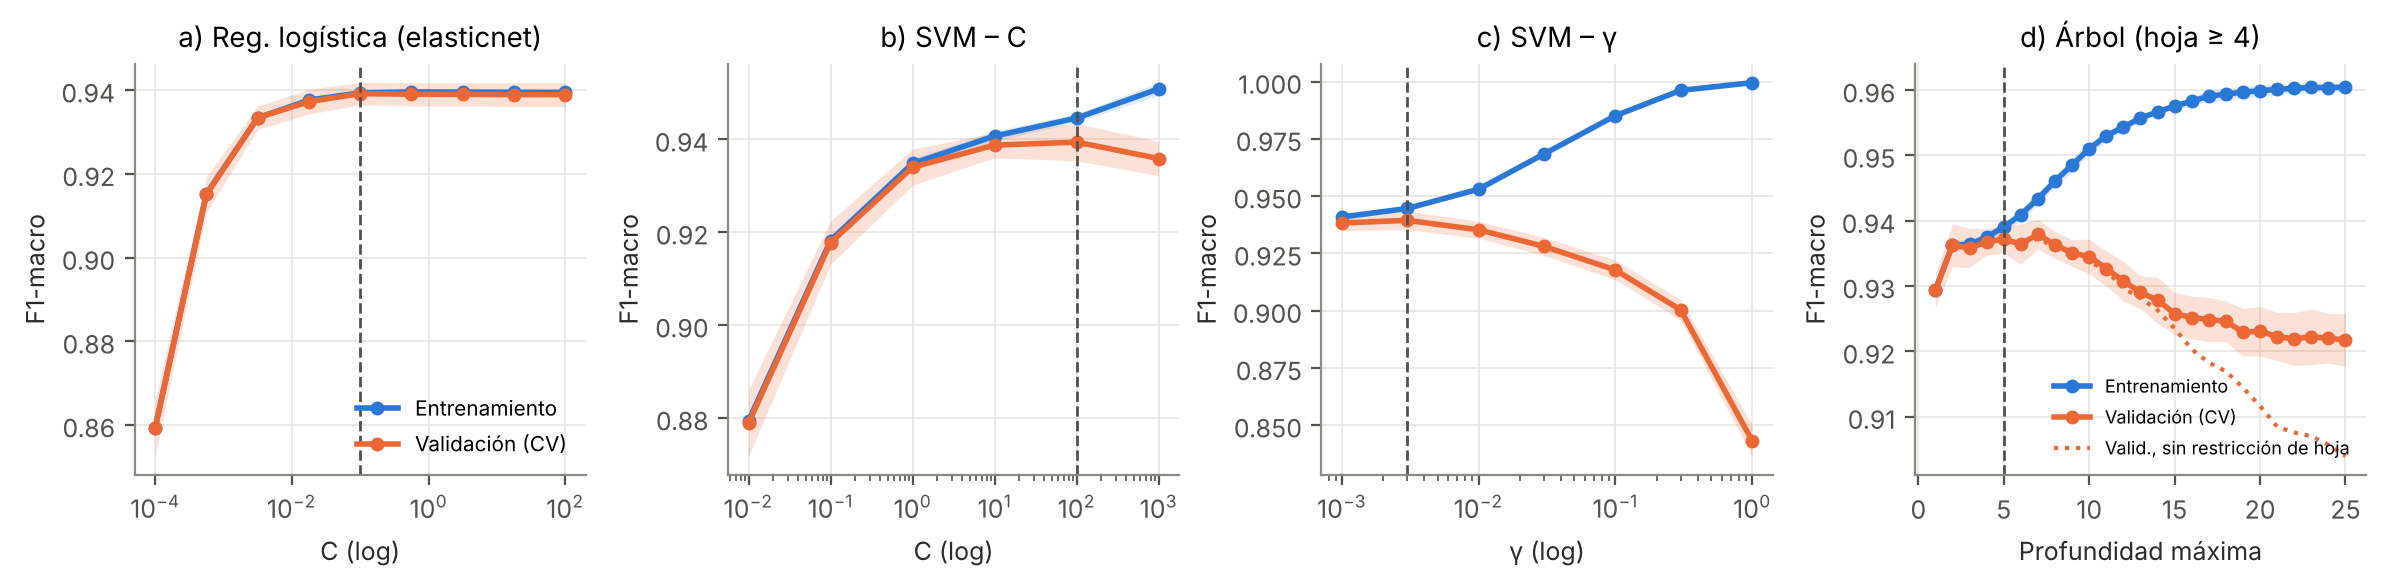
\includegraphics[width=0.93\textwidth]{fig4_complejidad_bin.png}
\caption{\label{fig:compl_bin}Curvas de complejidad del esquema binario. F1-macro medio de entrenamiento (azul) y validación (naranja) en CV de 5 \textit{folds}, con banda de $\pm 1$ desvío estándar; la línea vertical marca el valor elegido. (b--c) Calculadas sobre la submuestra de 10.000 registros. (d) Punteada: validación sin restricción de tamaño de hoja.}
\end{figure}

\subsection{Aplicación del modelo binario a los estudiantes en curso}\label{sec:curso}

Se usó la regresión logística ---con probabilidades bien calibradas y un desempeño equivalente al de los modelos más flexibles--- para estimar el riesgo de deserción de los 9762 estudiantes en curso con sus datos del primer año (Figura~\ref{fig:curso}). A diferencia de los casos de prueba, que se concentran en los extremos (el 91\,\% de los graduados tiene probabilidad $< 0{,}2$ y el 84\,\% de los desertores, $\geq 0{,}8$), los estudiantes en curso se reparten en todo el rango: el 29\,\% tiene riesgo bajo ($< 0{,}2$), el 45\,\% riesgo intermedio y el \textbf{26\,\% riesgo alto} ($\geq 0{,}8$; mediana 0,45). Este último grupo, que se parece a los desertores históricos, sería el candidato prioritario para acciones de acompañamiento. Como el desenlace de estos estudiantes se desconoce, estas estimaciones no pueden validarse con estos datos.

\begin{figure}[!htbp]
\centering
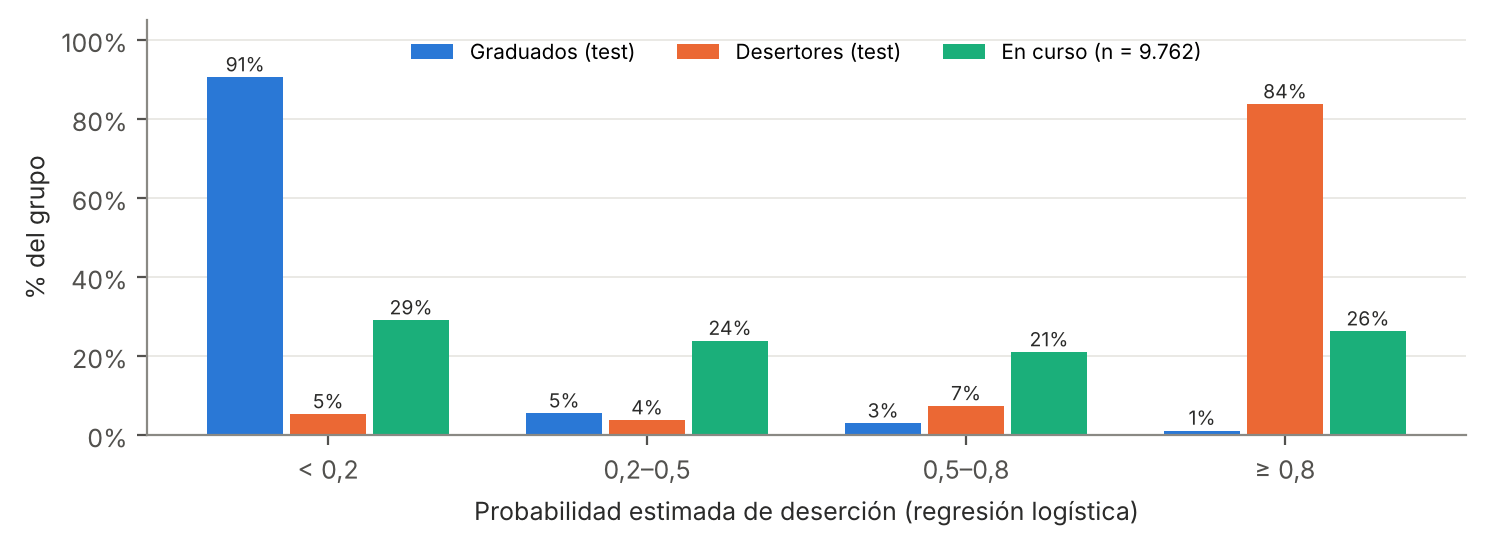
\includegraphics[width=0.66\textwidth]{fig_en_curso.png}
\caption{\label{fig:curso}Distribución de la probabilidad estimada de deserción (regresión logística binaria) por tramos de riesgo: graduados y desertores del conjunto de prueba (desenlace conocido) y estudiantes en curso (desenlace desconocido).}
\end{figure}

\subsection{Clasificación multiclase: desertor / en curso / graduado}

La Tabla~\ref{tab:multiclase} y la Figura~\ref{fig:mc}a resumen el desempeño en prueba. \textbf{XGBoost} obtiene el mejor F1-macro (0,789), accuracy (0,827) y AUC (0,934), seguido de cerca por \textbf{Random Forest} (F1-macro 0,787), que logra el mejor F1 en la clase En Curso (0,639) gracias a la ponderación balanceada de clases. Los modelos individuales quedan por debajo: el árbol de decisión (0,763) y K-NN (0,758), que además es el más afectado por la clase minoritaria. La regresión logística multinomial (0,777) supera a ambos y a su versión OvR (0,774), ya que la formulación multinomial estima las tres probabilidades de forma conjunta en vez de combinar tres clasificadores independientes no calibrados entre sí. La diferencia entre los dos mejores ensambles ($\approx$ 0,002) es menor que el desvío entre \textit{folds} ($\approx$ 0,005).

\begin{table}[!htbp]
\centering
\caption{Desempeño de los modelos multiclase en el conjunto de prueba}
\label{tab:multiclase}
\footnotesize
\setlength{\tabcolsep}{3.4pt}
\begin{tabular}{lcccccccc}
\toprule
\textbf{Modelo} & \textbf{Acc.} & \textbf{Prec.\ (m)} & \textbf{Rec.\ (m)} & \textbf{F1 (m)} & \textbf{AUC} & \textbf{F1 Des.} & \textbf{F1 Curso} & \textbf{F1 Grad.} \\
\midrule
K-NN                    & 0,800 & 0,773 & 0,751 & 0,758 & 0,909 & 0,825 & 0,582 & 0,867 \\
Árbol de decisión       & 0,808 & 0,774 & 0,757 & 0,763 & 0,914 & 0,841 & 0,574 & 0,876 \\
Reg.\ log.\ multinomial & 0,802 & 0,780 & 0,787 & 0,777 & 0,925 & 0,839 & 0,624 & 0,867 \\
Reg.\ log.\ OvR         & 0,804 & 0,777 & 0,778 & 0,774 & 0,918 & 0,836 & 0,615 & 0,871 \\
Random Forest (bagging) & 0,814 & 0,789 & \textbf{0,793} & 0,787 & 0,928 & 0,847 & \textbf{0,639} & 0,875 \\
AdaBoost (boosting)     & 0,821 & 0,789 & 0,776 & 0,781 & 0,917 & 0,852 & 0,608 & 0,884 \\
\rowcolor{orange!12}
XGBoost (boosting)      & \textbf{0,827} & \textbf{0,797} & 0,783 & \textbf{0,789} & \textbf{0,934} & \textbf{0,855} & 0,624 & \textbf{0,888} \\
\bottomrule
\end{tabular}

\vspace{2pt}
{\scriptsize $n_{\text{test}} = 9938$. Acc.\ = accuracy; (m) = promedio macro sobre las tres clases; AUC = AUC \textit{one-vs-rest} promedio macro; Des.\ = Desertor; Curso = En Curso; Grad.\ = Graduado; OvR = \textit{one-vs-rest}. En negrita, el mejor valor de cada columna.\par}
\end{table}

\begin{figure}[!htbp]
\centering
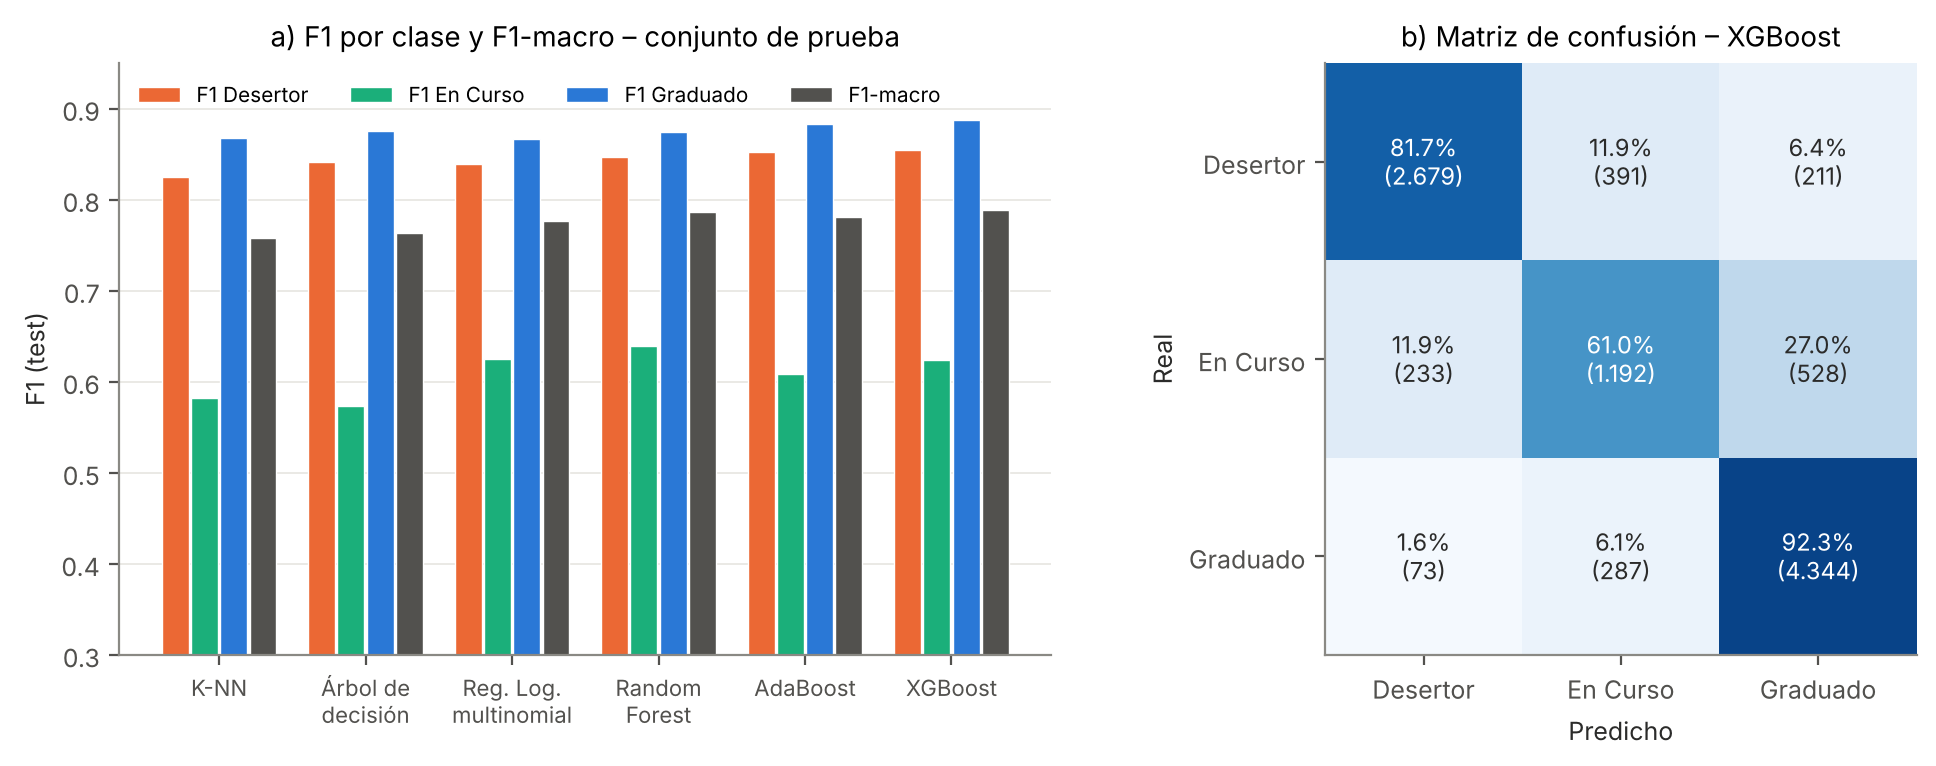
\includegraphics[width=0.85\textwidth]{fig5_mc_comp.png}
\caption{\label{fig:mc}Comparación de modelos multiclase y matriz de confusión del mejor modelo. (a) F1 por clase y F1-macro de cada modelo en el conjunto de prueba (el eje vertical comienza en 0,3). (b) Matriz de confusión de XGBoost normalizada por fila (clase real); entre paréntesis, número de estudiantes.}
\end{figure}

La matriz de confusión de XGBoost (Figura~\ref{fig:mc}b) muestra que el 92,3\,\% de los graduados y el 81,7\,\% de los desertores se clasifican correctamente, pero solo el 61,0\,\% de los estudiantes en curso: el 27,0\,\% se confunde con graduados y el 11,9\,\% con desertores. Los errores entre Desertor y Graduado son poco frecuentes (1,6\,\% de los graduados).

\textbf{Curvas de complejidad} (Figura~\ref{fig:compl_mc}). (a) En K-NN la complejidad \textbf{disminuye} al aumentar $k$: con $k = 1$ el F1-macro de entrenamiento es 1,0 y el de validación 0,69 (sobreajuste: el modelo memoriza el ruido); el óptimo de validación se alcanza con $k$ entre 21 y 41 ($\approx$ 0,75) y para $k > 100$ ambas curvas caen juntas (sub-ajuste). (b) En el árbol, la validación es máxima en profundidad 6--8 ($\approx$ 0,775) y luego desciende hasta 0,69, mientras el entrenamiento tiende a 1,0. (c) Random Forest, en cambio, \textbf{no se degrada} con la profundidad: aunque cada árbol profundo sobreajusta (entrenamiento $\approx$ 1,0), el promedio de 200 árboles decorrelacionados (\textit{bootstrap} + selección aleatoria de atributos) reduce la varianza y la validación se estabiliza en $\approx$ 0,79. (d) En XGBoost, con tasa de aprendizaje alta ($\eta = 0{,}3$) la log-loss de validación es mínima con $\sim$60 árboles y luego crece (de 0,44 a 0,57), mientras la de entrenamiento sigue bajando: el \textit{boosting} sobreajusta si se agregan iteraciones sin control. Con $\eta = 0{,}05$ el mínimo se alcanza cerca de los 470 árboles y la curva queda prácticamente plana, en línea con los 500 árboles seleccionados por CV.

\begin{figure}[!htbp]
\centering
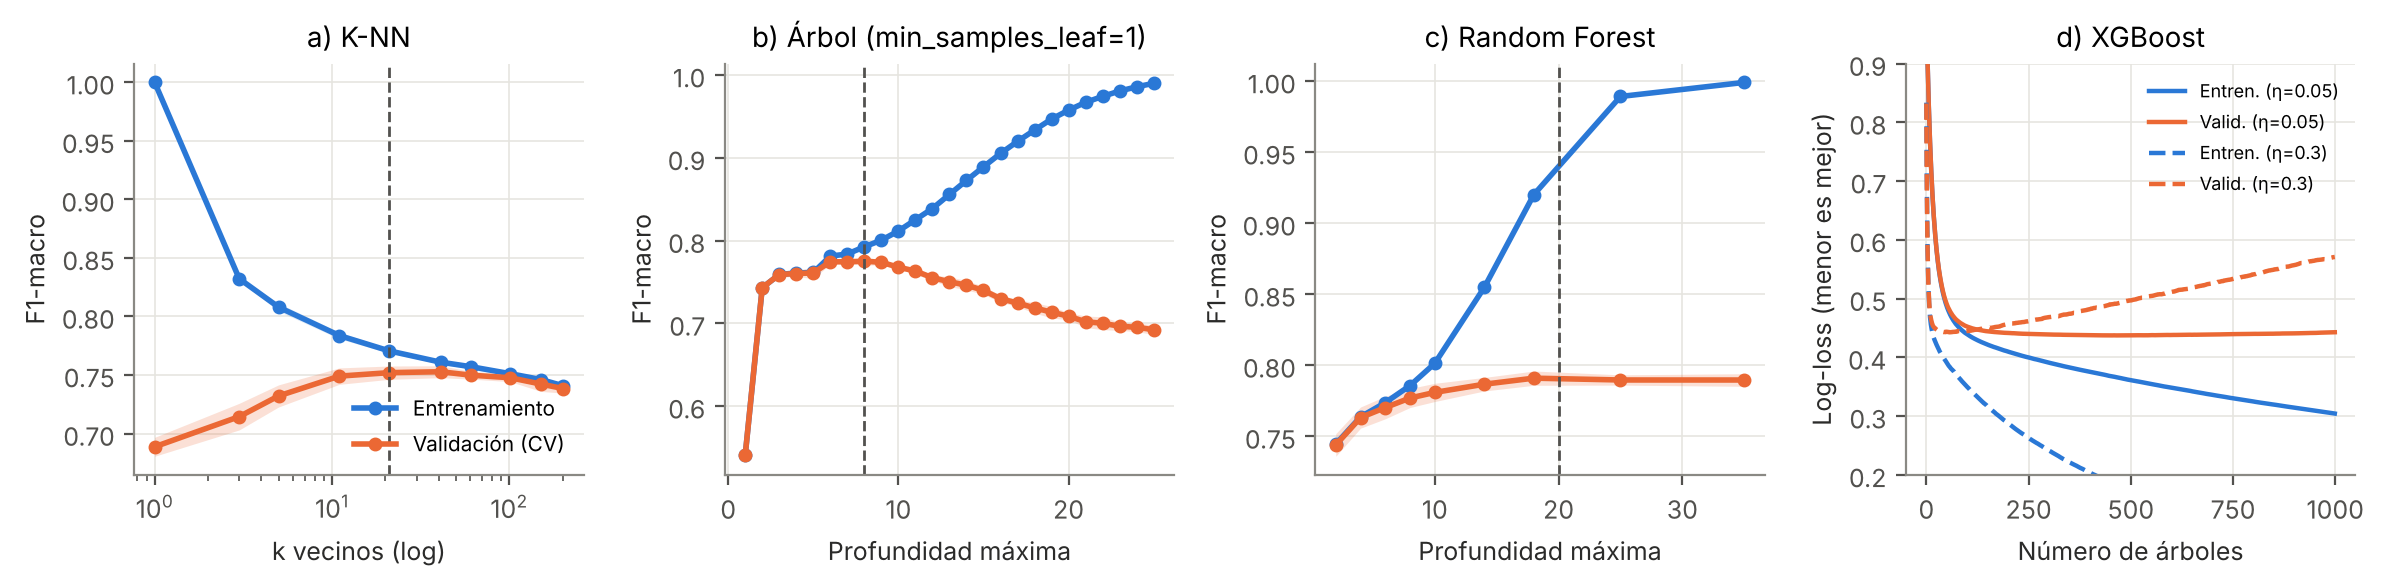
\includegraphics[width=0.93\textwidth]{fig6_complejidad_mc.png}
\caption{\label{fig:compl_mc}Curvas de complejidad del esquema multiclase. (a--c) F1-macro medio de entrenamiento (azul) y validación (naranja) en CV de 5 \textit{folds}, con banda de $\pm 1$ desvío estándar; la línea vertical marca el valor seleccionado. En K-NN la curva se calculó sobre una submuestra de 15.000 registros y en Random Forest con 200 árboles. (d) Log-loss multiclase de XGBoost en función del número de árboles para dos tasas de aprendizaje ($\eta$), evaluada sobre un 20\,\% del entrenamiento reservado como validación.}
\end{figure}

\subsection{Importancia de atributos en la tarea multiclase}

La importancia por permutación individual (Figura~\ref{fig:importancia}b) ubica a las \textbf{UC aprobadas en el 2.\textsuperscript{o} semestre} muy por encima del resto (caída del F1-macro de XGBoost de 0,194), seguidas por \textbf{tener la matrícula al día} (0,031). Sin embargo, el agrupamiento por correlación (Figura~\ref{fig:importancia}a) muestra tres bloques con $|\rho| > 0{,}5$: el académico (UC inscriptas y aprobadas y notas de ambos semestres), las evaluaciones de ambos semestres, y la nota de estudios previos con el puntaje de ingreso. Al permutar cada bloque completo (Figura~\ref{fig:importancia}c), el bloque académico produce una caída de \textbf{0,339}, 1,7 veces la de su variable más importante por sí sola (0,194): la permutación individual subestimaba su peso porque las variables del bloque se sustituyen entre sí. El orden del resto se mantiene ---matrícula al día (0,033), evaluaciones (0,030), carrera, edad y beca---, y las variables demográficas y del entorno familiar no aportan (caídas $\leq 0{,}002$).

\begin{figure}[!htbp]
\centering
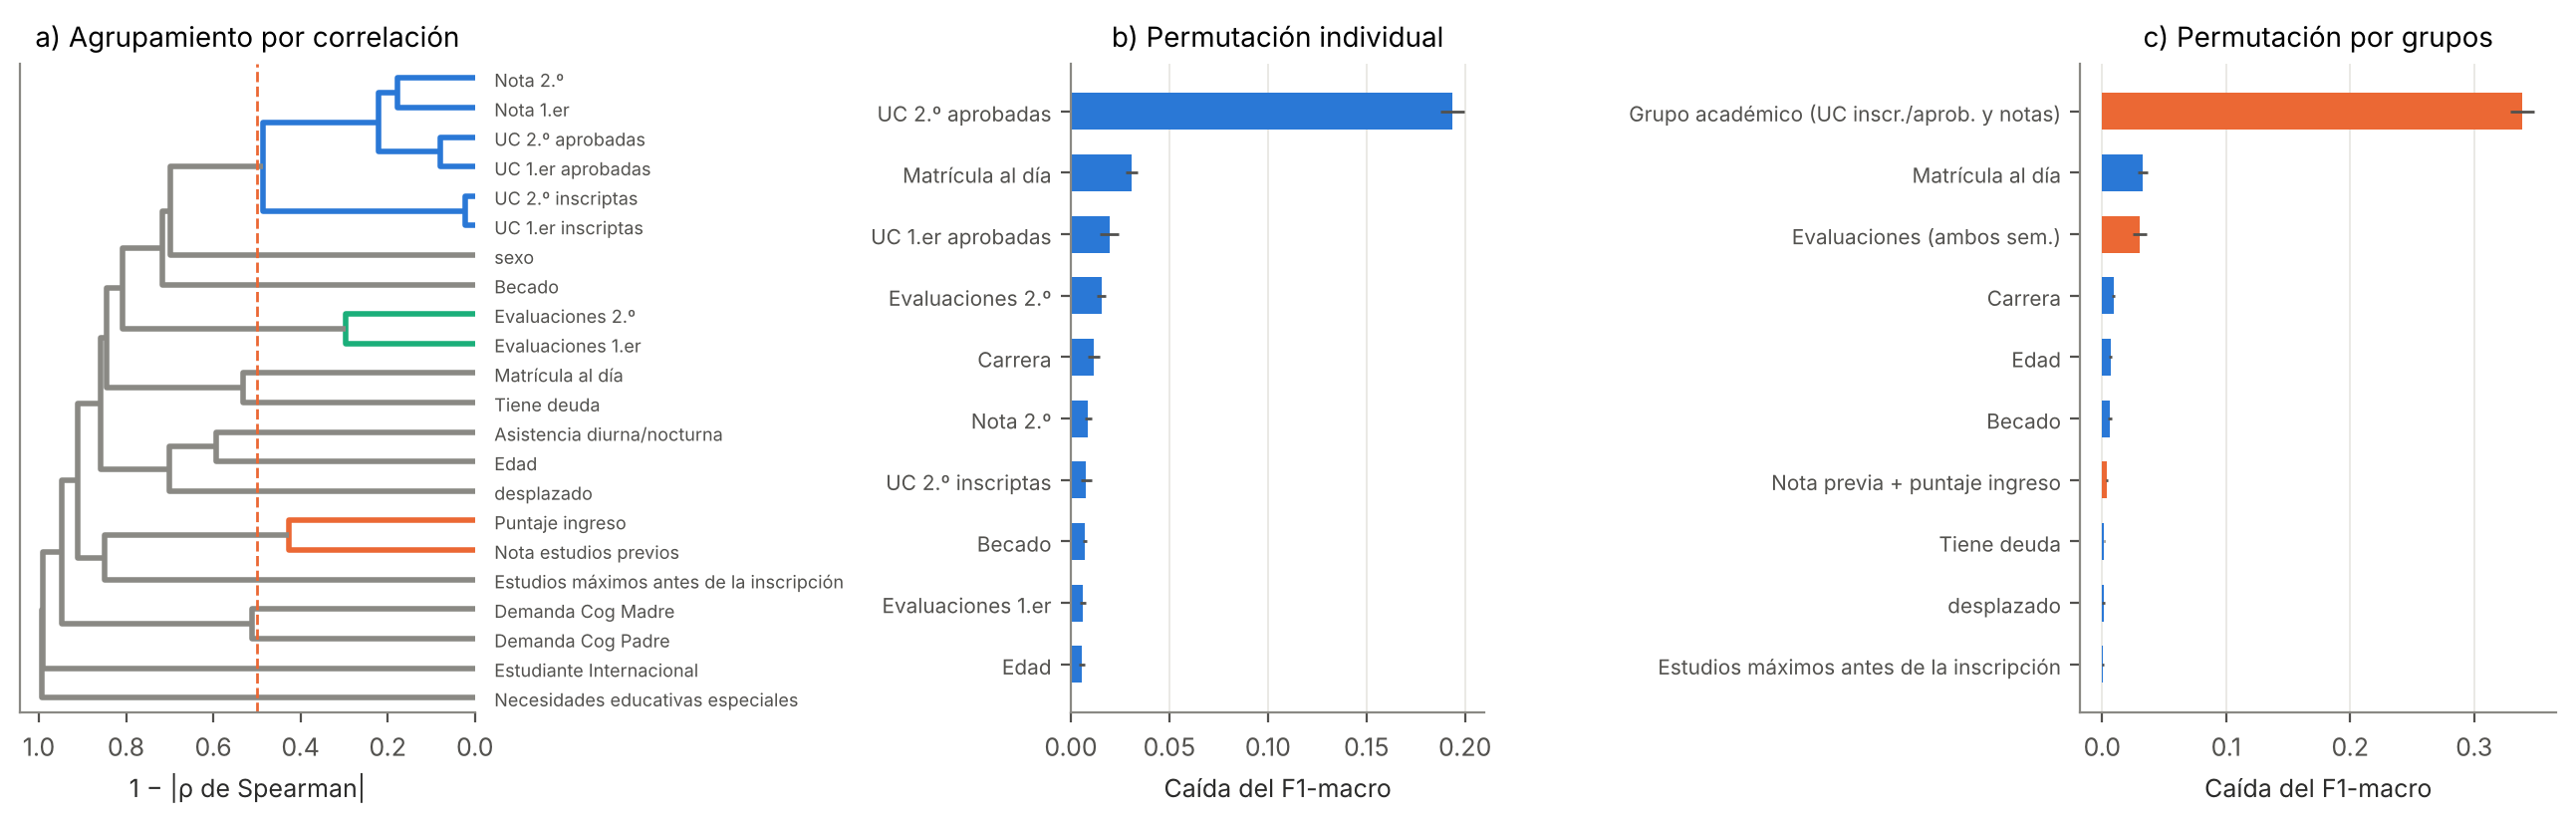
\includegraphics[width=0.95\textwidth]{fig7_importancia_grupos.png}
\caption{\label{fig:importancia}Importancia de atributos en el esquema multiclase (XGBoost). (a) Dendrograma del clustering jerárquico sobre la correlación de Spearman entre atributos; en color, los grupos con $|\rho| > 0{,}5$ (línea discontinua). (b) Disminución media del F1-macro al permutar cada variable por separado. (c) Ídem permutando cada grupo completo (naranja = grupo de varias variables). 5 repeticiones sobre 5000 registros de prueba; barras de error = $\pm 1$ desvío estándar. UC = unidades curriculares.}
\end{figure}


\subsection{Modelo explicativo de la deserción}\label{sec:explicativo}

En el conjunto reducido de predictores la correlación máxima entre variables numéricas es $|\rho| = 0{,}39$ y el VIF máximo, 2,2, por lo que los coeficientes pueden interpretarse. La curva de complejidad (Figura~\ref{fig:explicativo}a) muestra que el F1-macro de validación se estabiliza desde $C \approx 0{,}01$, con entrenamiento y validación superpuestos; la regla de 1 SE elige $C = 0{,}01$, que retiene \textbf{10 de las 20 variables} con un F1-macro de validación de 0,925 (0,926 el máximo). En prueba, el modelo reajustado alcanza F1-macro = 0,925 y AUC = 0,970, apenas por debajo de la LR completa (0,937 y 0,976) con la mitad de las variables. La trayectoria de coeficientes (Figura~\ref{fig:explicativo}b) muestra que el índice de rendimiento es la primera variable en entrar al modelo y conserva el mayor efecto bajo cualquier regularización, seguido por la morosidad, la beca y las evaluaciones. La importancia por permutación (Figura~\ref{fig:explicativo}c) lo confirma: permutar el índice reduce el F1-macro en 0,326, la morosidad en 0,048 y las evaluaciones en 0,011; el resto, menos de 0,005.

\begin{figure}[!htbp]
\centering
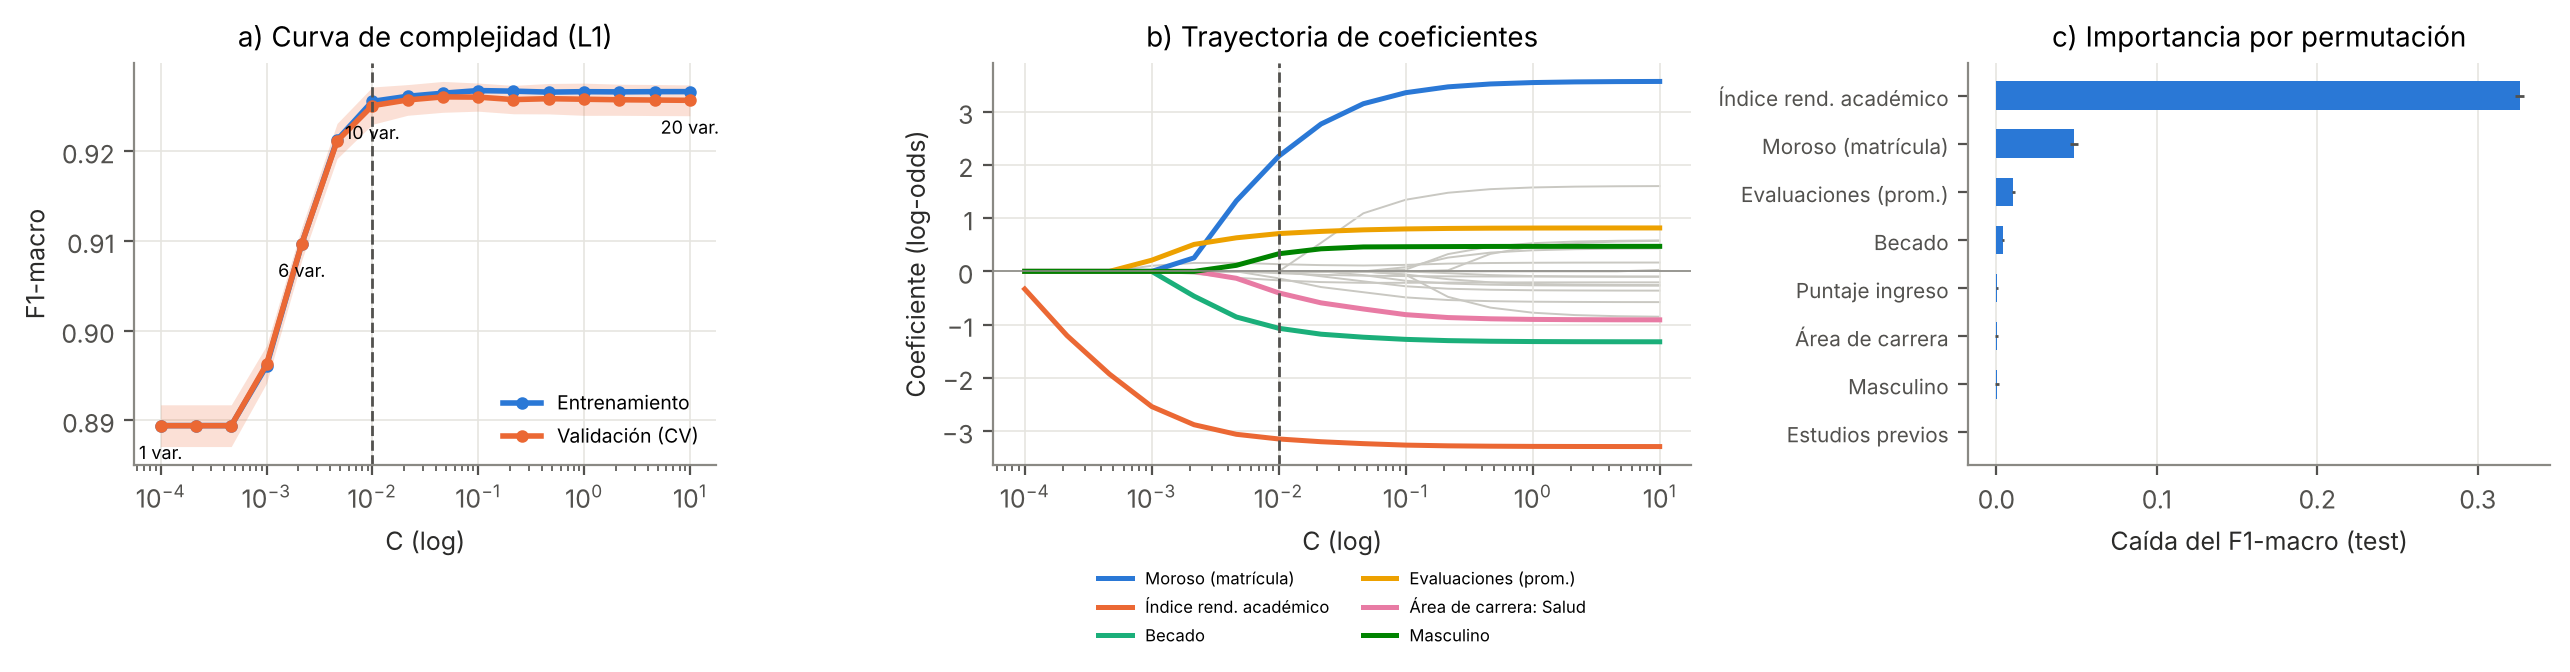
\includegraphics[width=\textwidth]{fig_explicativo.png}
\caption{\label{fig:explicativo}Modelo logístico explicativo. (a) Curva de complejidad de la regularización L1: F1-macro de entrenamiento y validación (CV de 5 \textit{folds}, banda = $\pm 1$ error estándar) y número de variables retenidas. (b) Trayectoria de los coeficientes en función de $C$; en color, las seis variables con mayor efecto. La línea discontinua marca el $C$ elegido por la regla de 1 SE. (c) Caída del F1-macro en prueba al permutar cada variable (10 repeticiones).}
\end{figure}

\begin{table}[!htbp]
\centering
\caption{Regresión logística explicativa reajustada sobre las 10 variables retenidas por Lasso}
\label{tab:explicativo}
\footnotesize
\begin{tabular}{lccccc}
\toprule
\textbf{Variable} & $\boldsymbol{\beta}$ & \textbf{Error est.} & \textbf{OR} & \textbf{IC 95\,\% del OR} & \textbf{Valor p} \\
\midrule
Moroso (matrícula no al día; sí vs.\ no)  & $+3{,}57$ & 0,14 & 35,6 & 26,9--47,0 & $<0{,}001$ \\
Índice de rendimiento académico (1 sd)     & $-3{,}29$ & 0,04 & 0,04 & 0,03--0,04 & $<0{,}001$ \\
Becado (sí vs.\ no)                        & $-1{,}31$ & 0,07 & 0,27 & 0,24--0,31 & $<0{,}001$ \\
Evaluaciones rendidas, promedio (1 sd)     & $+0{,}80$ & 0,03 & 2,22 & 2,10--2,35 & $<0{,}001$ \\
Área: Salud                                & $-0{,}75$ & 0,07 & 0,47 & 0,41--0,55 & $<0{,}001$ \\
Masculino (vs.\ femenino)                  & $+0{,}62$ & 0,05 & 1,86 & 1,68--2,06 & $<0{,}001$ \\
Área: Comunicación, marketing y diseño     & $-0{,}45$ & 0,06 & 0,64 & 0,56--0,72 & $<0{,}001$ \\
Puntaje de ingreso (1 sd)                  & $-0{,}23$ & 0,02 & 0,80 & 0,76--0,84 & $<0{,}001$ \\
Edad al inscribirse (1 sd)                 & $+0{,}09$ & 0,02 & 1,10 & 1,05--1,15 & $<0{,}001$ \\
Nivel ocupacional de la familia (1 sd)     & $-0{,}09$ & 0,02 & 0,91 & 0,87--0,96 & $<0{,}001$ \\
\bottomrule
\end{tabular}

\vspace{2pt}
{\scriptsize $\beta$ = coeficiente en log-odds de desertar; OR = \textit{odds ratio} $= e^{\beta}$. Variables continuas estandarizadas (efecto de +1 desvío estándar); indicadores 0/1 sin estandarizar. Área de carrera: respecto de la categoría de referencia (Administración y turismo), que agrupa también a las áreas que el Lasso no retuvo. Entrenamiento: $n = 31.940$. IC aproximados: no corrigen por la selección de variables.\par}
\end{table}

La Tabla~\ref{tab:explicativo} cuantifica los efectos manteniendo constantes las demás variables. Tener la matrícula impaga multiplica la chance (\textit{odds}) de desertar por 36, mientras que cada desvío estándar adicional del índice de rendimiento la reduce a menos de una vigésima parte (OR = 0,04). La beca protege (OR = 0,27) y ser varón aumenta el riesgo (OR = 1,86). A igual rendimiento, rendir más evaluaciones aumenta la chance de desertar (OR = 2,22), lo que sugiere que reflejan instancias desaprobadas o recursadas más que esfuerzo. Las áreas de Salud y Comunicación tienen menor riesgo que el resto. La dependencia parcial (Figura~\ref{fig:pdp_exp}) traduce estos efectos a probabilidades: la probabilidad de desertar cae de forma sigmoide con el índice de rendimiento, pero para un estudiante de rendimiento promedio (índice $\approx 0$) es de 0,92 si está moroso y de 0,38 si tiene la matrícula al día; de 0,52 en varones y 0,41 en mujeres; y de 0,36 en Salud frente a 0,49 en el resto de las áreas.

\begin{figure}[!htbp]
\centering
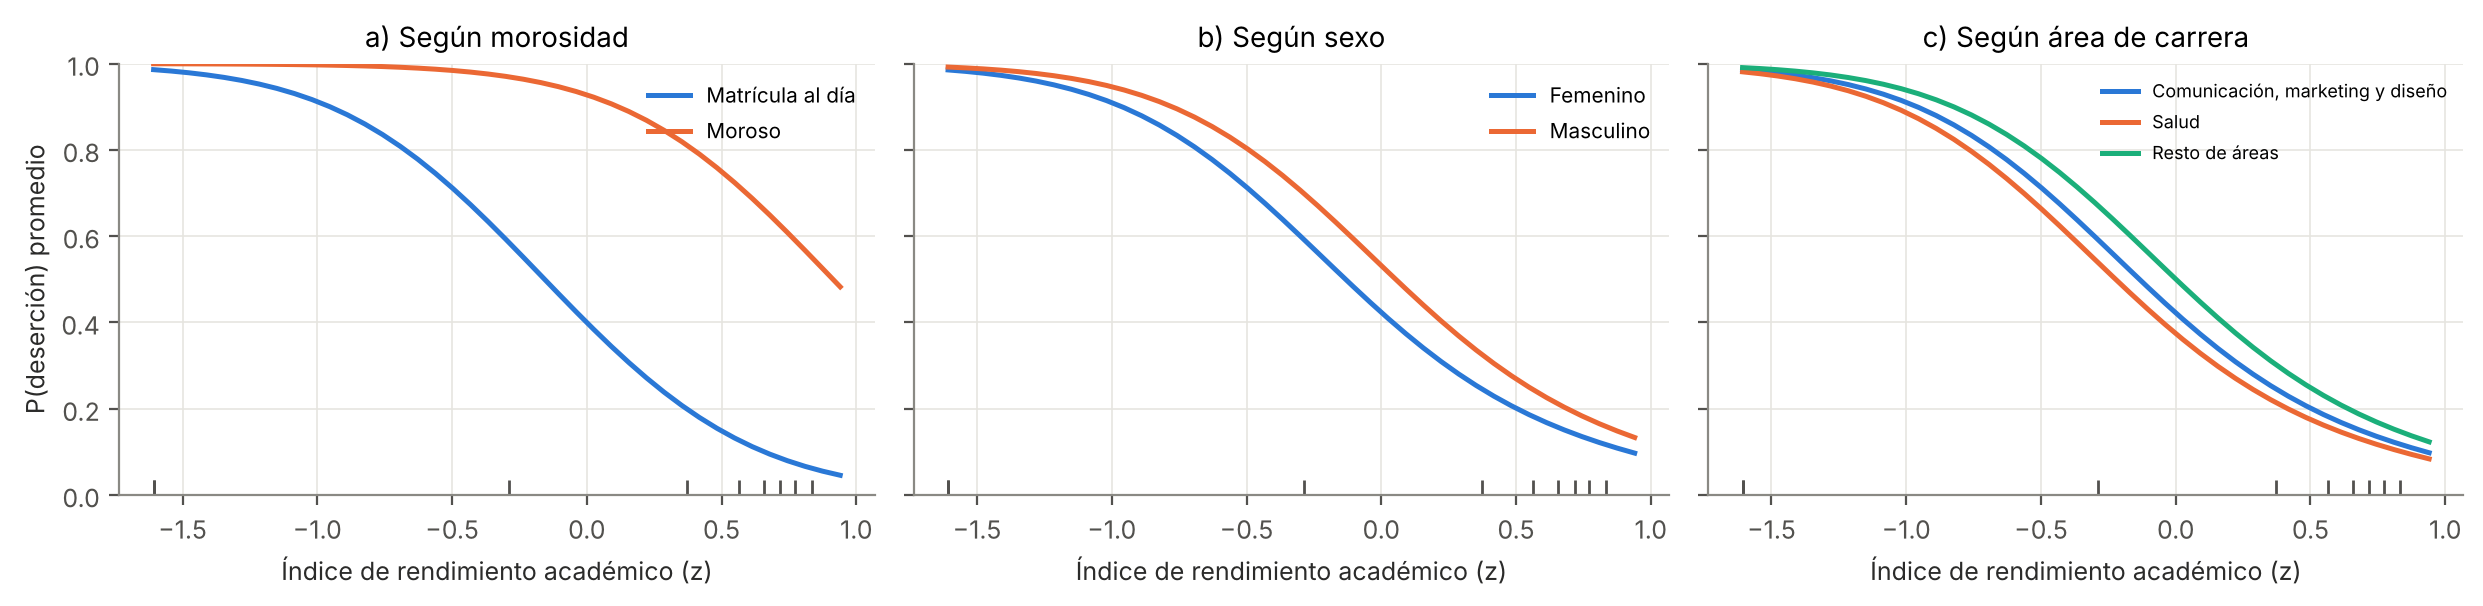
\includegraphics[width=\textwidth]{fig_pdp_explicativo.png}
\caption{\label{fig:pdp_exp}Dependencia parcial del modelo explicativo: probabilidad predicha de deserción en función del índice de rendimiento académico, fijando cada valor de (a) la morosidad, (b) el sexo y (c) el área de carrera, y promediando sobre los demás atributos (3000 registros de prueba). Las marcas sobre el eje horizontal son los deciles del índice. ``Resto de áreas'' = áreas sin efecto propio en el modelo.}
\end{figure}

% =====================================================================
\section{Discusión}\label{sec:discusion}

Los resultados abordan la deserción desde tres perspectivas. Para \textbf{predecir}, todos los modelos binarios distinguen graduados de desertores con F1-macro $\approx$ 0,94 y AUC $\approx$ 0,97, y aplicados a los estudiantes en curso identifican a un 26\,\% con riesgo alto; para \textbf{describir}, la tarea multiclase muestra que ``en curso'' es un estado intermedio difícil de reconocer; y para \textbf{explicar}, el rendimiento académico y la morosidad dominan, seguidos por la beca y el sexo, lo que respalda H1. Esto es coherente con la integración académica de Tinto (1975, 1993), con el peso de los factores financieros en Bean (1980) y Bean y Metzner (1985), con la relevancia del primer año señalada por Yorke y Longden (2004) y con Kim et al.\ (2023), que sobre el dataset original reportan AUC entre 0,93 y 0,96 y a las UC aprobadas como predictor principal.

En la tarea binaria, la regresión logística iguala a los modelos flexibles (H2): su curva de complejidad no muestra brecha entre entrenamiento y validación, la SVM y el árbol solo rinden mejor con baja complejidad y el modelo explicativo con 10 variables pierde muy poco desempeño. Por eso la elegimos a la vez para estimar el riesgo de los estudiantes en curso y para explicar el fenómeno: ofrece probabilidades calibradas y coeficientes interpretables con la misma precisión. El \textit{Voting} no aportó mejoras porque sus componentes cometen casi los mismos errores. En la multiclase, en cambio, los ensambles de árboles superaron a los modelos individuales (H3), porque separar la clase intermedia requiere interacciones no lineales que el \textit{bagging} y el \textit{boosting} estabilizan; K-NN fue el más débil, ya que con 47 atributos mixtos la distancia pierde significado. La dificultad de ``en curso'' (F1 $\approx$ 0,60--0,64), también observada en el dataset original (Martins et al., 2021), es esperable: su desenlace todavía no ocurrió. Ese mismo carácter intermedio aparece en la aplicación del modelo binario, donde el 45\,\% de estos estudiantes recibe una probabilidad intermedia.

Las variables correlacionadas exigieron cuidado en la interpretación: la permutación individual subestimaba el bloque académico (0,194 frente a 0,339 al permutarlo completo), y por eso el modelo explicativo resume ese bloque en un único índice. Las principales \textbf{limitaciones} son cuatro. Primero, parte de la señal puede ser consecuencia y no causa de la deserción: un estudiante que ya abandonó no aprueba materias ni paga la matrícula, lo que explica IV $> 0{,}5$ y un OR de 36 para la morosidad; los coeficientes describen asociaciones, no efectos causales. Segundo, la aplicación a los estudiantes en curso no puede validarse con estos datos y supone que se parecen a las cohortes históricas; requiere validación prospectiva y debe usarse como insumo para el acompañamiento, no como decisión automática. Tercero, los datos provienen de una única institución y fueron aumentados sintéticamente, por lo que el desempeño puede estar sobreestimado. Cuarto, por costo computacional la SVM se ajustó con una submuestra y los IC del modelo explicativo no corrigen la selección de variables.

% =====================================================================
\section{Conclusión}\label{sec:conclusion}

En base a nuestros resultados, podemos concluir que una regresión logística regularizada permite resolver de manera confiable la tarea de distinguir a los estudiantes que desertarán de los que se graduarán (F1-macro = 0,937; AUC = 0,976) a partir de los datos disponibles al cierre del primer año, con el mismo desempeño que modelos más complejos, y que puede aplicarse a los estudiantes en curso para priorizar acciones de acompañamiento; que, para distinguir además la categoría ``en curso'', los ensambles de árboles ---en particular XGBoost (F1-macro = 0,789)--- son la mejor opción, aunque esa clase sigue siendo difícil de reconocer; y que el rendimiento académico y la morosidad en la matrícula son los factores más asociados a la deserción, seguidos por la beca y el sexo.

% =====================================================================
\section*{Bibliografía}\label{sec:bibliografia}
\addcontentsline{toc}{section}{Bibliografía}

\begin{footnotesize}
\begin{list}{}{\setlength{\leftmargin}{1.2em}\setlength{\itemindent}{-1.2em}\setlength{\itemsep}{0pt}\setlength{\parsep}{0pt}}
\item Bean, J. P. (1980). Dropouts and turnover: The synthesis and test of a causal model of student attrition. \textit{Research in Higher Education}, 12(2), 155--187.
\item Bean, J. P. y Metzner, B. S. (1985). A conceptual model of nontraditional undergraduate student attrition. \textit{Review of Educational Research}, 55(4), 485--540.
\item Breiman, L. (2001). Random forests. \textit{Machine Learning}, 45(1), 5--32.
\item Chen, T. y Guestrin, C. (2016). XGBoost: A scalable tree boosting system. \textit{Proceedings of the 22nd ACM SIGKDD International Conference on Knowledge Discovery and Data Mining}, 785--794.
\item Kim, S., Yoo, E. y Kim, S. (2023). Why do students drop out? University dropout prediction and associated factor analysis using machine learning techniques. \textit{arXiv preprint} \href{https://arxiv.org/abs/2310.10987}{arXiv:2310.10987}.
\item Martins, M. V., Tolledo, D., Machado, J., Baptista, L. M. T. y Realinho, V. (2021). Early prediction of student's performance in higher education: A case study. En \textit{Trends and Applications in Information Systems and Technologies (WorldCIST 2021)}, Advances in Intelligent Systems and Computing, vol.\ 1365, 166--175. Springer.
\item OECD (2019). \textit{Education at a Glance 2019: OECD Indicators}. París: OECD Publishing.
\item Pedregosa, F. et al. (2011). Scikit-learn: Machine learning in Python. \textit{Journal of Machine Learning Research}, 12, 2825--2830.
\item Realinho, V., Machado, J., Baptista, L. y Martins, M. V. (2022). Predicting student dropout and academic success. \textit{Data}, 7(11), 146.
\item Reade, W. y Chow, A. (2024). Classification with an Academic Success Dataset. \textit{Kaggle Playground Series}, Season 4, Episode 6.
\item Tinto, V. (1975). Dropout from higher education: A theoretical synthesis of recent research. \textit{Review of Educational Research}, 45(1), 89--125.
\item Tinto, V. (1993). \textit{Leaving College: Rethinking the Causes and Cures of Student Attrition} (2.ª ed.). Chicago: University of Chicago Press.
\item Yorke, M. y Longden, B. (2004). \textit{Retention and Student Success in Higher Education}. Maidenhead: Open University Press / SRHE.
\end{list}
\end{footnotesize}

\end{document}
